\documentclass[]{risa}

\usepackage[figuresright]{rotating}
\usepackage{url}
\usepackage{graphicx}
\usepackage{float}
\usepackage{multicol}
\usepackage{color} 
\usepackage{amsmath}
\usepackage[official]{eurosym}
\begin{document}

\jvol{}
\jnum{}
\pubyear{}

\doi{}
\copyright{2009 Society for Risk Analysis}
\issnyear{}

\title[Back to normal?]{Back to normal? A method to test and correct the impact of a shock on healthcare usage frequency data}

\author[David Mori\~na et al.]{David Mori\~na$^{1}$,\affiliation{Department of Econometrics, Statistics and Applied Economics, Universitat de Barcelona, Riskcenter-IREA, dmorina@ub.edu}
%%
Amanda Fern\'andez-Fontelo$^{2}$,\affiliation{Department of Mathematics, Universitat Aut\`onoma de Barcelona}
%%%
Montserrat Guill\'en$^{1}$\affiliation{Department of Econometrics, Statistics and Applied Economics, Universitat de Barcelona, Riskcenter-IREA}
} 

\begin{abstract}
A method based on Bayesian structural time series is proposed to predict healthcare usage trends and to test for changes in the series levels during or after an abnormal year, such as that of the 2020 COVID-19 pandemic. Our method can also be used to calculate correction factors for frequency count data that can then be integrated in a preprocessing step before undertaking any statistical analysis, and, in this way, the impact of a shock can be eliminated. Here, adjustments are derived for a large private health insurer in Spain from estimates of average healthcare usage. Levels in 2020 were 12\% down on 2019 figures, but rose in 2021 and 2022, when the average usage was 16 and 22\% higher, respectively, than in 2019. Our approach is shown to outperform traditional time series techniques, including the root mean square and the mean absolute percentage errors, resulting in more accurate predictions and lower error measures. Healthcare insurance usage did not fully recover and is still above pre-pandemic levels in 2022, with the exception of some patient groups and specific medical services, which might be one of the reasons for the recent increase in insurance premiums. The method developed can be implemented in other areas of risk analysis concerned with frequency counts and which are exposed to shocks.
\end{abstract}

\begin{keywords}
health services; modelling; Poisson offset; covid-19; time series; pre-processing
\end{keywords}

\maketitle

\section{Introduction}\label{intro}
Following the events of 2020, one of the main problems faced by health insurers is that historical count records of the use of medical services – which usually serve as the basis for the yearly update of future prices – have become heavily influenced by the pandemic shock \cite{kim2022impact, xu2021impact, cantor2022impact}. This poses the question as to whether pandemic data remain useful for future projections. If rescaling were feasible, then these data could still be analyzed, net, that is, of the pandemic effect; if not, data from pandemic and post-pandemic years may not be comparable to those from more normal periods.

Here, we seek to measure the impact of the COVID-19 pandemic shock in terms of the frequency of use of medical insurance services. Moreover, we take advantage of these estimates to correct individual portfolio data since 2020 for statistical modeling in the subsequent years, so that no data have to be discarded. In so doing, we draw on traditional time series decomposition methods, in which shocks can be identified and deducted from the original series in order to derive future trends net of the shock.

After a shock such as that of the COVID-19 pandemic, analysts might be tempted to delete the information for the years 2020 to 2022, and return to using 2019 as their baseline, on the grounds that once things are back to normal, this should be everyone’s reference year. However, the consequences of having to reschedule medical treatment and preventive care in 2020, which may have led to an overuse of medical services in 2021, and possibly 2022, are still unclear \cite{wilensky2022covid}. It might even be the case that some medical specialties have suffered the effects more than others, indicating that the post-pandemic impact may still be significant for some specific medical use records. During the pandemic, hospitals had to ride the various waves of the pandemic, but on-going cancer treatments, including chemotherapy and surgeries, were discontinued as little as possible. Yet, many non-urgent surgeries, preventative care appointments, and diagnostic services were canceled, resulting in delayed treatment and an increased healthcare burden for patients with non-COVID related conditions. And it is this that may have had a potential long-term effect on usage counts.

We present a method based on the analysis of count time series that captures the shock in 2020 and provides much better forecasts for 2021 and 2022 than that provided by traditional methods. Our approach is helpful for measuring the impact of the pandemic in terms of the excess (or dearth of) frequency of claims, and can be used to test whether or not usage frequencies have returned to the normal levels of 2019. Moreover, once the size of the pandemic shock has been calculated, data analysts can choose to study post-pandemic data without the impact of this shock by simply introducing an adequate scale correction.

In a case study of a large insurance company in Spain, we find that health insurance claims during the pandemic (2020) were about 12\% down on pre-pandemic figures (2019), while in 2021 and 2022, the usage of health care services increased but has yet to return to 2019 levels. There are, however, a number of exceptions to this general result. For instance, the series of frequency claims for people aged $>$ 60 has returned to the 2019 average, whereas some services, such as visits to a general practitioner (GP), were 48\% higher in 2022 than in 2019.

\subsection{Background}
After the outbreak of COVID-19 in 2020, a number of lessons have been learned. Yet, the pandemic caused an unprecedented disruption to the global health insurance market \cite{przybytniowski2022risk, szczygielski2022impact}. First and foremost, it obliged many people to stay home, so that the number of medical appointments, hospital admissions, and other medical services in 2020 were initially down on 2019 figures. 

The fall in the frequency of claims for healthcare usage can be attributed to the postponement of elective medical procedures, such as surgeries and other invasive treatments, which are typically covered by health insurance. These procedures were often put on hold due to the strain that the healthcare system was under, as well as the mobility restrictions in many areas. Likewise, the fear of contracting COVID-19 in healthcare settings led some to avoid seeking medical care, even for serious conditions that would typically require health insurance coverage. Overall, it has been reported that the decrease in health insurance claims during the pandemic was attributable to a combination of these factors \cite{plott2020unexpected}, but that a rebound was expected after the pandemic. The resilience of health insurance systems to the impact of contagious diseases like COVID-19 has been recently discussed from a theoretical approach \cite{}.

The pandemic created a state of emergency across all areas of healthcare, resulting in reduced resources for the treatment of other illnesses. This pattern was similar in many countries around the globe \cite{xu2021impact, mogharab2022global}, but there is evidence that some demographic groups were more badly affected than others. For example, older adults in the Netherlands \cite{mizee2022delay} and Germany \cite{michalowsky2021effect} suffered substantially higher cancellation rates of medical visits and the postponement of medical care in 2020 than younger adults. In this regard, several studies discuss the consequences of delaying the treatment of non-emergency diseases \cite{kim2022impactb, kotrych2022delay, di2022impact} and scheduled surgeries \cite{ricciardiello2021impact}.

In general, in many countries, private health insurance enjoyed something of a boost after 2020 as the market expanded, with a price hike in premiums and a considerable rise in the number of policyholders. One reason why premiums rose, despite the fact that the initial effect of COVID-19 was a reduction in claims, is that the pandemic changed the approach of health insurance companies to risk after what had previously been considered a potential risk presented itself as a veritable catastrophe \cite{richter2020covid}. Indeed, many insurers opted to take a more cautious approach to risk after COVID-19, resulting in higher premiums, increased deductibles, and reduced coverage. Additionally, some insurers have changed their eligibility criteria and now charge higher premiums for those with pre-existing conditions. The pandemic has also triggered an increase in the cost of healthcare services \cite{poisal2022national}, reflecting the higher demand, and increased costs for both medical supplies and the delivery of care. As a result, many health insurance companies have increased their prices. A further trigger has been the greater uncertainty surrounding a possible increase in claims due to the fact that some pathologies that might otherwise have been diagnosed, were not. In these instances the treatment is likely to be more expensive than had the disease been identified in its early stages. Furthermore, reports of the long-term effects of COVID-19 have also raised fears of a protracted increase in the level of claims.



\subsection{Motivation and objectives}
Many analysts realize that the years 2020, 2021, and 2022 can be deemed special in terms of health insurance; moreover, experts are also  unclear about the effects of retaining these data in long-term risk analyses \cite{biancalana2022quantitative}. Besides the catastrophic effect they might have on insurability and contract design in all lines of business \cite{hartwig2020insurance}, the problem is identifying whether the fluctuations in claims frequency and severity have stabilized after 2021. In this regard, a tool that can correct claim frequency information based on a quantitative assessment of the under-/over-reporting of claims is of particular interest so that future analyses can be based on the data corresponding to the most recent years instead of having to resort to 2019 data.

Here, we propose a method to meet the following three objectives: 1) the quantification of the impact of a shock on claim frequency series, 2) the determination as to whether a claim frequency series continues to show a significant impact of that shock, and 3) the rescaling of frequency data to eliminate the effects of the impact.

We illustrate our method with data drawn from a Spanish private health insurance company. We seek to quantify the effect of the pandemic outbreak on the time series of claims, by identifying the size of that shock in 2020 and the return to the pre-pandemic level of 2019. To do so, we design a step-by-step procedure that can help health insurers decide whether or not their portfolio information continues to be affected by the pandemic shock. In this way, they will know if the claims data are suitable for use in their predictive modeling, or, should the data continue to present signs of a post-pandemic effect, they can determine the size of this distortion and how the data might be corrected to make it suitable for accurate premium calculations. The analytical procedure we propose can be conducted with all types of claim, as well as by subgroups defined by claimant characteristics, including sex and age, and by type of healthcare service.



\section{Methods and data}\label{methods}
Here, we propose an approach that adapts the well-known difference-in-differences methodology to the time series setting. We do so by explicitly modeling the counterfactual of a time series observed both before and after the occurrence of an event of interest, potentially impacting the evolution of the process, the case, in this instance, of the shock provoked by the COVID-19 pandemic. Our approach provides a fully Bayesian time-series estimate of the effect and uses model averaging to construct the most appropriate synthetic control for modeling the counterfactual.

\subsection{Shock impact detection and evaluation}\label{methodsBSTS}
Let $y_t$ denote the observation $t$ in a real-valued time series. A structural time series (STS) model can be described by a pair of equations relating $y_t$ to a vector of latent state variables $\alpha_t$:

\begin{equation}\label{eq1}
y_t = Z_t^T \alpha_t + \epsilon_t, \epsilon_t \sim N(0, H_t)
\end{equation}
\begin{equation}\label{eq2}
\alpha_{t+1} = T_t \alpha_t + R_t \eta_t, \eta_t \sim N(0, Q_t).
\end{equation}

Equation~\ref{eq1} or the observation equation links the observed data $y_t$ with the unobserved latent state $\alpha_t$; whereas Equation~\ref{eq2} or the transition equation defines how the latent state $\alpha_t$ evolves over time. A model that can be described by these two equations is said to be in state space form, which defines a large class of models including the autoregressive integrated moving average or ARIMA \cite{scott_predicting_nodate}. 

In this work, $y_t$ is a vector representing the evolution in the weekly number of claims associated with a private health insurance company, $Z_t$ is a $d$-dimensional output vector, $T_t$ is a $d \times d$ transition matrix, $R_t$ is a $d \times q$ control matrix, $\epsilon_t$ is a scalar observation error with noise variance $H_t$, and $\eta_t$ is a $q$-dimensional system error with a $q \times q$ state-diffusion matrix $Q_t$ , where $q \leq d$. 

Let $\theta$ denote the set of all model parameters and $\alpha = (\alpha_1, \ldots, \alpha_m)$ denote the full state sequence. Following \cite{brodersen_inferring_2015}, a prior distribution $p(\theta)$ is specified on the model parameters jointly with a distribution $p(\alpha_0 \mid \theta)$ on the initial state values. We then sample from $p(\alpha, \theta \mid y)$ using a Markov chain Monte Carlo (MCMC) algorithm. To estimate the impact of a shock on the evolution of a time series based on the methodology proposed, draws of the model parameters $\theta$ and the state vector $\alpha$ given the observed data $y_1, \ldots, y_n$ in the training period are simulated. We denote $y_1, \ldots, y_n$ as  $y_{1:n}$. The posterior simulations are then used to simulate from the posterior predictive distribution $p(\tilde{y}_{n+1:m} \mid y_{1:n})$ over the counterfactual time series $\tilde{y}_{n+1:m}$ given the observed pre-shock activity $y_{1:n}$. Finally, we use the posterior predictive samples to compute the posterior distribution of the pointwise impact $y_t - \tilde{y}_t$ for each $t=(n+1), \ldots, m$ and the posterior distribution of cumulative impact, summarized by their median,  which can be interpreted as the shock level, and its 95\% credible intervals (CI). When using the Bayesian methodology described to estimate the parameters, the method is usually referred to as a Bayesian structural time series (BSTS).


As shown below, this methodology is also capable of providing accurate forecasts. Its performance is compared to that of usual time series modelling, such as ARIMA (see for instance\cite{shumway_arima_2017}) by means of two commonly used error measures - that is, the root mean square error (RMSE) and the mean absolute percentage error (MAPE) -, computed according to Equations~\ref{eq3} and~\ref{eq4} respectively. We assume that $n^*$ periods are forecast, and we denote the observed values $O_j$ and the forecast values $F_j$, with $j=1,\dots, n^*$.

\begin{equation}\label{eq3}
RMSE=\sqrt{\frac{1}{n^*} \cdot \sum_{j=1}^{n^*} (O_j-F_j)^2},
\end{equation}

\begin{equation}\label{eq4}
MAPE=\frac{100}{n^*} \sum_{j=1}^{n^*} \left | \frac{O_j-F_j}{O_j} \right |.
\end{equation}

\subsection{Implications for pre-processing data net of a shock impact in GLM frequency modelling}

The BSTS-estimated median shock level can later be used to pre-process data when filtering out the effect of the impact of the pandemic shock. In time series decomposition, the value equal to the estimated factor impact can be extracted from the series $y_t$ before modeling future trends. In predictive modeling, when individual data on observed claims and claimant covariate information are available, the estimated shock level can be combined with individual exposures. In this way, the expected claim frequency corresponds to what would be expected once the impact of the pandemic effect has been removed.

Let us introduce the notation of cross-sectional data at time $T$. Suppose that $N_{iT}$ is the observed number of claims for policyholder $i$ in year $T$, where $i=1,\dots, N_T$ and $N_T$ is the number of policyholders in year $T$. Assume that a vector of $K+1$ characteristics $x_{iT}$ is available for individual $i$ in year $T$ where the first component is a constant and $\nu_{iT} \in (0,1]$ denotes exposure, i.e. the fraction of the whole year when the policy was valid, then predictive modeling of the expected number of claims usually establishes that $E(N_{iT}|x_{iT}, \nu_{iT})= \nu_{iT}\mu(x_{iT})$, where $\mu$ is a function that links the effect of the covariates to the expected number of claims, provided that this effect is proportional to exposure \cite{wuthrich2023statistical}. In the Poisson model, $\mu(x_{iT})=\beta^\prime x_{iT}$, with $\beta = (\beta_0,...,\beta_K)$ a vector of parameters to be estimated, where $\beta_0$ is an intercept.

If the impact of the pandemic shock has to be eliminated from these data for the purpose of predictive modeling and making comparisons between years, then the expected number of claims should be affected by a change and this can easily be achieved through the exposure component. Therefore new individual exposures $\nu^*_{iT}$ can be defined so that
$$
\nu^*_{iT}=\nu_{iT} \times m_T
$$
where $m_T=1+f_T$ is obtained from the Bayesian estimate described in the previous section, which can be expressed as a percent change, $f_T$. 

Note that $f_T$ refers to the cumulated posterior distribution median relative change. A positive $f_T$ means that the shock has produced an excess of counts, corresponding to increased exposure. A negative $f_T$ means that the shock has reduced the number of counts, corresponding to decreased exposure. Note that $f_T$ may be a global correction that is equal for all individuals, or it may have been calculated by subgroups, so that it could change by individual. We have opted to drop the $i$ subindex in order to eliminate complex notation from the methodology.

Once the corrected exposures, $\nu^*_{iT}$, are used in the Poisson model estimation process, the model outcome is net of the pandemic shock impact. Below we illustrate how this can be implemented.

In this illustration, we have incorporated the Bayesian estimates into the individual exposures and fitted Poisson regression models for claims frequency in a simple example with portfolio data sets before, during,  and after the pandemic shock. We compare analyses of single vs multiple-year predictive modeling, with and without the inclusion of the shock correction, and show that predictive claim models for pre- and post-pandemic yearly portfolios are actually comparable. Some additional results, including the comparison of the distribution of the predicted number of claims per individual with and without the pandemic effect, reveal a persistent change in the distribution. The analysis by groups of individuals, also shows that processing before eliminating the pandemic effect need not be homogeneous for the whole portfolio.

Figure~\ref{fig1} provides a summary of our approach.
\begin{center}
  \begin{figure}[ht]
	%\begin{minipage}{80mm}
    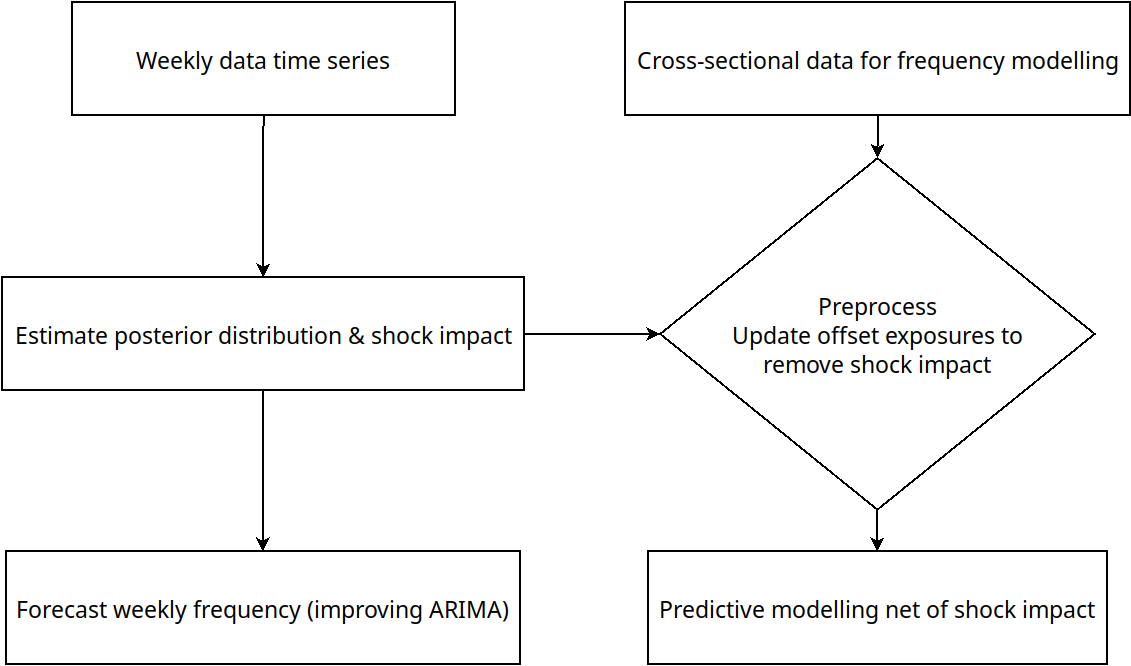
\includegraphics[width=8cm, height=5cm]{Diagrama1.png}\caption{Methodology for testing the impact of a shock and, afterwards, filtering the data.}\label{fig1}
		%\end{minipage}
  \end{figure}
	\end{center}
	

\subsection{Data}\label{data}
We observed the weekly number of medical claims associated with a private health insurance scheme run by one of the largest companies in Spain from the beginning of 2019 to the end of 2022, by type of service, province, sex and age group. The overall monthly number of contracts was also taken into account, to control for observed trends unrelated to the consequences of pandemic claims. To make the latter weekly, we performed a linear interpolation process.

A weekly frequency count corresponds to the number of claims reported to the insurance company in the course of one week. A claim refers to the use of a medical service, such as a visit to a GP, a blood test, an x-ray, surgery, a visit to a specialist, the use of an ambulance or treatment in an emergency room or hospital that was covered by the insurance policy.

The insurer providing us with its data was affected by the enforcement of social distance measures, adopted in Spain as in many other countries. These triggered a sudden fall in the frequency of health insurance claims and this decrease, moreover, was substantial given that during the lock-downs in 2020 people reduced their normal activities and canceled preventive medical visits, while medical services were primarily focused on treating COVID-19 patients. Thus, the insurance company’s portfolio initially fell markedly in 2020, affected in all probability by the impact of the death of a certain number of policyholders during the pandemic. Then, as in other European countries, the portfolio grew substantially owing to the saturation of the public health system. The latter situation raised grave concerns among many citizens who opted to underwrite private health insurance to protect themselves and their families in case of a global medical service collapse. Although private hospitals, accessible to holders of a health insurance contract, were also relatively saturated during the pandemic, COVID-19 mainly impacted public hospitals.

The immediate impact of the COVID-19 pandemic can be quantified by comparing the number of claims in 2019 and 2020, while the medium- and long-term consequences can be quantified by comparing the number of claims in 2019, with those in 2021 and 2022. To illustrate the ability of the methodology proposed to quantify the impact of the pandemic on the use of  private health services, in what follows we describe in detail the evolution in medical claims globally, by sex, among those aged over 60 and in the three Spanish provinces that are home to the country’s largest cities (that is, Madrid, Barcelona, and Valencia). A number of specific services of particular interest are also analyzed.

In addition to what we specifically report here, two other scenarios were also considered as regards the definition of the post-pandemic period that we then compare with the normal period (01-01-2019 to 13-03-2020) and the pandemic period (14-03-2020 to 21-06-2020). In the first approach we compare the period 01-01-2019 to 21-06-2020 with the period 22-06-2020 to 31-12-2021, whereas in the second, we exclude the pandemic period and compare the period 01-01-2019 to 13-03-2020 with the period 21-06-2020 to 31-12-2021. These results are available on request from the authors.

The R code used to generate the results and figures described below are available in the GitHub repository \url{https://github.com/dmorinya/BSTS_HealthInsurance}. The results can be reproduced with the cardiology subset. The rest of our data cannot be made publicly available due to owner restrictions. All coding has been done in R software \cite{r_core_team_r_2019}, using the packages \textit{bsts} \cite{scott_predicting_nodate} and \textit{CausalImpact}\cite{brodersen_inferring_2015}. 
	
\begin{center}
  \begin{figure*}[h]
	\begin{minipage}{160mm}
    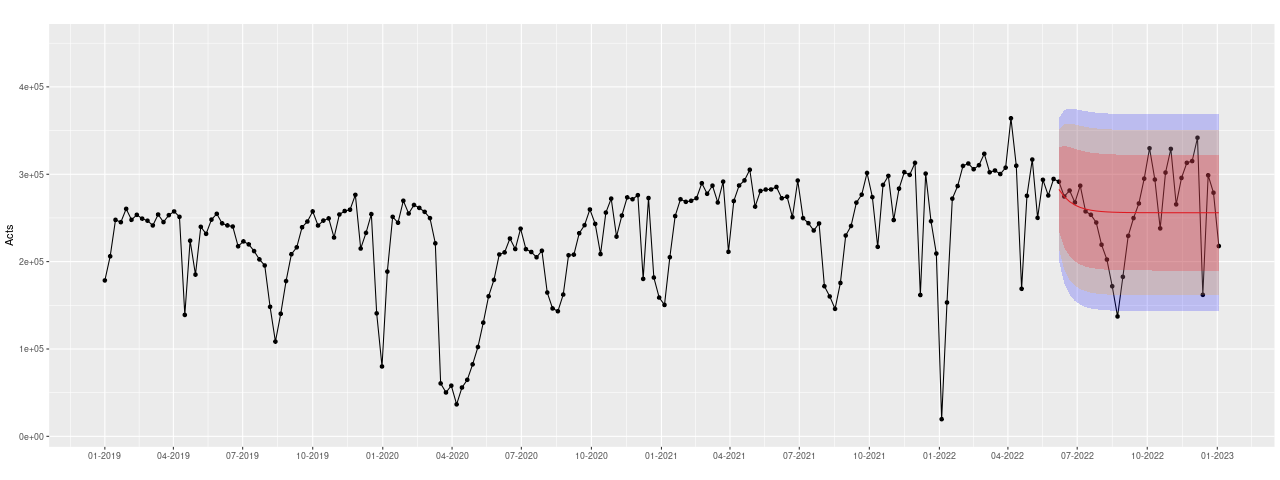
\includegraphics[width=16cm]{arima_global_prediction.png}\caption{Number of weekly claims (black) and the ARIMA-based forecast for the period July-December 2022 (red), 95\% confidence bands in light blue, 90\% confidence bands in light purple and 75\% confidence bands in light pink.}\label{fig2}
	 \end{minipage}
  \end{figure*}
	\end{center}

\begin{center}
  \begin{figure*}[h]
	\begin{minipage}{160mm}
    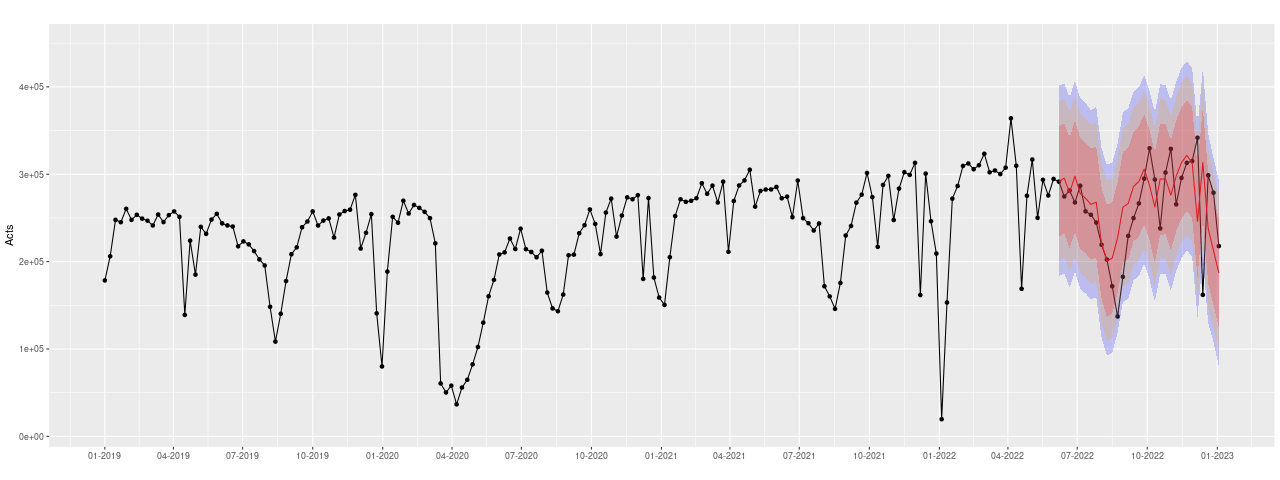
\includegraphics[width=16cm]{bsts_global_prediction.png}\caption{Number of weekly claims (black) and BSTS forecast for the period July-December 2022 (red), 95\% credible bands in light blue, 90\% credible bands in light purple and 75\% credible bands in light pink.}\label{fig3}
  \end{minipage}
  \end{figure*}
\end{center}

\section{Results}\label{results}
Although the impact of the COVID-19 pandemic on the usage of health insurance services could be calculated as the reduction in claims frequency observed in 2020 with respect to 2019 and the increase observed in 2021 and 2022, also with respect to 2019, this information could not then simply be used to forecast the future behavior of claims. Indeed, in the case study we conduct here, we could simply state that a total of 11,754,419 claims (recall this corresponds to the whole portfolio of a large insurance company, where a claim is defined as any medical service provided, including for example a blood test) were made in 2019, while 10,305,088 were made in 2020, 13,337,053 in 2021 and 14,129,286 in 2022. That is, a decrease of 12\% was recorded in 2020 and increases of some 13 and 20\% were recorded, respectively, in 2021 and 2022, compared in both cases to 2019. However, on the basis of these figures, data analysts cannot then predict future usage trends. Moreover, these figures are affected by an increase of new policy holders from 2020 onwards. 


A more sophisticated approach, and one that would allow analysts to make a forecast of future behavior, is provided by the classical ARIMA time series models, ignoring the fact that the original series is not stationary (Kwiatkowski–Phillips–Schmidt–Shin test p-value of 0.02) %and it is unclear as to how to make it stationary using the Box-Jenkins methodology. 
When fitting the best ARIMA model, based on Akaike’s Information Criterion (AIC), to the period January 2019 to June 2022 – that is an AR(1) process – the weekly frequency of claims forecast produced for the period July 2022 to December 2022 is shown in Figure~\ref{fig2}. 

It is evident that the ARIMA-based forecast is only capable of capturing the mean of the process, but at the price of considerable discrepancies between observed and forecast values (RMSE of 50,094 and MAPE of 17.28\%). The forecast for the same period provided by the BSTS approach outlined above is shown in Figure~\ref{fig3}. Here, it is clear that the forecast produced is much more accurate than that provided by the classical approach. Indeed, in this case, the RMSE is around 48,388 and the MAPE is around 15.59\%; thus, in both instances the error is lower than when adopting the classical ARIMA-based approach.



Table~\ref{tab1} reports the estimated effect – both the median and 95\% credible intervals – of the pandemic shock on the overall weekly time series of claims frequency observations and by group of policy holders, geographical area and medical specialty.

\begin{table*}[ht]
\centering
\def\~{\hphantom{0}}
\begin{minipage}{160mm}
\caption{BSTS estimated median percentage change attributable to impact of the pandemic and post-pandemic over the frequency usage of health insurance associated services.}
\label{tab1}
  \begin{tabular*}{\textwidth}{ccccccc}
    \Hline
    & \multicolumn{2}{c}{2019-2020} & \multicolumn{2}{c}{2019-2021} & \multicolumn{2}{c}{2019-2022}\\
    \hline
    & Difference (95\% CI) & p-value & Difference (95\% CI) & p-value & Difference (95\% CI) & p-value\\
    \hline
    Total & -12\% (-16\%, -7\%) & 0.0004 & 16\% (7.5\%, 37\%) & 0.00255 & 22\% (9.1\%, 63\%) & 0.00431\\
    \hline
    Females & -12\% (-16\%, -6.8\%) &	0.00038 & 15\% (6.3\%, 39\%) & 0.00378 & 22\% (8\%, 64\%) & 0.00591\\
    Males & -13\% (-17\%, -7.4\%) & 0.00026 & 16\% (8\%, 37\%) &	0.00237 & 22\% (11\%, 60\%) & 0.00304\\
    \hline
    Over 60 & -20\% (-24\%, -14\%) & 0.00002 & -7.2\% (-15\%, 18\%) & 0.08928 & 1\% (-11\%, 49\%) & 0.21511\\
    \hline
    Oncology &  -11\% (-17\%, -4.7\%) &	0.0025 & 8.4\% (-1.9\%, 32\%) & 0.04785 & 15\% (-0.99\%, 65\%) & 0.03075\\
    Cardiology & -10\% (-15\%, -4.8\%) & 0.00172 & 18\% (6.1\%, 39\%) & 0.00593 & 26\% (8.4\%, 61\%) & 0.0068\\
    Obstetrics & -12\% (-16\%, -7.1\%) & 0.00027 & 11\% (0.88\%, 28\%) & 0.01976 & 16\% (0.75\%, 44\%) & 0.02215\\
    Urology & -11\% (-15\%, -5.3\%) & 0.00097 & 19\% (6.7\%, 43\%) & 0.00536 & 28\% (8.8\%, 68\%) & 0.00622\\
    General medicine & 2.2\% (-2.8\%, 8.1\%) & 0.20173 & 28\% (20\%, 51\%) & 0.0001 & 48\% (37\%, 91\%) & 0.00004\\
    Osteopathy & -23\% (-27\%, -18\%) & 0.00002 & 12\% (1.8\%, 29\%) & 0.01566 & 31\% (17\%, 63\%) & 0.00301\\
    \hline
    Madrid & -16\% (-20\%, -10\%) & 0.00008 & 4.5\% (-3.6\%, 25\%) & 0.12841 & 11\% (-0.58\%, 47\%) & 0.02908\\
    Barcelona & -8.9\% (-14\%, -2.6\%) & 0.00792 & 25\% (14\%, 60\%) & 0.0003 & 33\% (16\%, 96\%) & 0.00135\\
    Valencia & -8.8\% (-13\%, -3.1\%) & 0.00487 & 29\% (19\%, 54\%) & 0.00046 & 39\% (25\%, 85\%) & 0.00034\\
    \Hline
\end{tabular*}
\end{minipage}
\end{table*}

As can be seen, a quite remarkable reduction was recorded in the usage of health insurance services in 2020 compared to the previous year (with the exception of general medicine services), while the consequences of this reduction are already evident in most cases in 2021, most notably in urology and general medicine. The 2.2\% increase estimated for general medicine in 2020 (and a part of the 28 and 48\% increases reported, respectively, for 2021 and 2022) can be attributed to the fact that some of the COVID-19 testing was conducted by this service. Geographically, the behavior of Barcelona and Valencia is largely similar in both comparisons, while Madrid records a greater reduction in usage in 2020 and smaller increases in both 2021 and 2022. This might reflect the fact that Madrid has an older exposure profile; yet, this hypothesis cannot be confirmed with the data available as the monthly number of contracts is aggregated only at the national level. The behavior of both sexes is also very similar, but the reduction in usage among individuals aged over 60 in 2020 is significantly greater than that of the general population. Moreover, in this group, no increase in usage was recorded in 2021 (indeed, we find a reduction of around 7\%, although it is non-significant, and a slight increase of around 1\% in 2022, again non-significant). Here, it should be borne in mind that COVID-19-associated mortality rates were much higher among this subpopulation; thus, it is reasonable to expect that the older adults ($>$ 60) that survived are healthier than in the past and that their need for health services is not as great as that of older adults in 2019.


To illustrate how the Bayesian estimates provided by the proposed methodology can be incorporated in data preprocessing, we next fit several Poisson regression models to the number of cardiology claims (i.e. a visit to a cardiologist) by age ($30-60$/$>60$) and sex (male/female). We fit one model per year (2019, 2020, 2021, and 2022) and a global model including data for all the years under consideration. Additionally, we fit a Poisson regression model using an offset correction accounting for the global Bayesian estimates reported in Table~\ref{tab1} (i.e. -12\% for 2020, 16\% for 2021, and 22\% for 2022) and a further Poisson regression model using specific Bayesian estimates for each subgroup of age and sex. The estimates yielded by each of these models are shown in Table~\ref{tab2}. The differences are immediately evident, especially in the case of the impact of the age group parameter when using specific corrections. Note that this model reflects the expected claims net of the impact of the pandemic. Thus, when all years are combined and the shock is filtered out, the incidence in adults aged $>$ 60 is 2.03 times greater than that in adults aged 30 to 60, while the incidence in men is 20\% higher than that in women. A year-by-year analysis without any shock correction reveals lower incidence rates in general, but in particular for 2022.


\begin{table*}[ht]
\centering
\def\~{\hphantom{0}}
\begin{minipage}{160mm}
\caption{Parameter estimates of incidence rate ratios for Poisson regression modeling of the frequency of claims originating in a cardiology service (p-values correspond to testing incidence rate equal to 1) for policyholders aged 30+. A correction refers to a change in exposure before estimating the Poisson regression using the BSTS impact estimate for 2020, 2021, and 2022 either globally, the same for all individuals, or by gender/age group. A correction eliminates the impact of the pandemic shock.}
\label{tab2}
  \begin{tabular*}{\textwidth}{ccccccc}
    \Hline
    Model & $e^{\hat{\beta}_0}$ (p-value) & $e^{\hat{\beta}_\text{Sex (Male)}}$ (p-value) & $e^{\hat{\beta}_\text{Age (60+)}}$ (p-value) & Sample size\\
    \hline
    Only 2019 &  0.60 ($< 0.0001$) & 1.15 ($< 0.0001$) & 1.74 ($< 0.0001$) & 75,218 \\
    Only 2020 &  0.57 ($< 0.0001$) & 1.14 ($< 0.0001$) & 1.68 ($< 0.0001$) & 73,477 \\
    Only 2021 &  0.64 ($< 0.0001$) & 1.15 ($< 0.0001$) & 1.63 ($< 0.0001$) & 86,737 \\
    Only 2022 &  0.66 ($< 0.0001$) & 1.15 ($< 0.0001$) & 1.59 ($< 0.0001$) & 91,188 \\
    Full sample (without correction) &  0.62 ($< 0.0001$) & 1.15 ($< 0.0001$) & 1.65 ($< 0.0001$) & 
		 326,620 \\
    %Full sample (without correction and year adjusted) & -0.11 ($< 0.0001$) & 0.03 ($< 0.0001$) & 0.31 ($< 0.0001$) \\
    Full sample (with global correction) & 0.58 ($< 0.0001$)   & 1.15 ($< 0.0001$) & 1.67 ($< 0.0001$) & 
		 326,620 \\
    Full sample (with specific correction) & 0.51 ($< 0.0001$) & 1.20 ($< 0.0001$)  & 2.03 ($< 0.0001$) & 
		 326,620 \\
\Hline
\end{tabular*}
\end{minipage}
\end{table*}


\begin{table*}[ht]
\centering
\def\~{\hphantom{0}}
\begin{minipage}{160mm}
\caption{Observed and expected distribution of number of cardiology claims in each Poisson regression model considered.}
\label{tab3}
  \begin{tabular*}{\textwidth}{cccccccc}
    \Hline
    Model & 0 claims & 1 claim & 2 claims & 3 claims & 4 claims & 5 or more claims \\
    \hline
    Observed  & 150,670 & 120,040 & 38,283 & 11,499 & 3,861 & 2,267 \\ 
    Full sample (without correction) & 150,562.9 & 113,790.0 & 45,585.7 & 13,008.4 & 2,977.5 & 695.5 \\
    Full sample (with global correction) & 158,908.3 & 111,823.1 & 41,812.7 & 11,163.0 & 2,394.6 & 518.2 \\
    Full sample (with specific correction) & 163,809.8 & 108,088.0 & 40,061,1 & 11,289.5 & 2,688.8 & 682.8 \\
\Hline
\end{tabular*}
\end{minipage}
\end{table*}

Table~\ref{tab3} shows that the observed data are best fitted by the Poisson regression model without any correction, whereas those incorporating global and specific corrections model (with less and more detail, respectively) the counterfactual that the impact of the COVID-19 pandemic is negligible. This indicates that insurance companies can use all the information to compare the temporal behavior of usage series, without having to exclude any specific year. Moreover, note that the last row of Table \ref{tab3} shows what the outcome distribution would have been in the absence of the pandemic shock. Indeed, the full sample model with this specific correction reports the expected behavior net of the pandemic shock, and comparison with the uncorrected full sample reveals how the estimated incidences impact the final premiums.


If cost information is available, the approach proposed can be used to estimate annual costs in the absence of the shock. In our case, if we assign an average unit cost of 50€ per visit to the cardiology service, Table~\ref{tab3} shows that the accumulated cost of cardiology visits over the period 2019–2022 is around 12,975,500€. Actual annual costs were 3,020,850€ in 2019; 2,704,550€ in 2020; 3,489,900€ in 2021, and 3,760,200€ in 2022. Using the global adjustment, the total cost in the absence of the pandemic can be estimated at 12,184,867€, which implies an excess cost equal to 790,633€ (i.e. 12,975,500€ - 12,184,867€). When incorporating the specific age/gender correction, the estimated excess cost is equal to 987,116€.




The usage made of other services, including that of general medicine, was also analyzed as described above for cardiology, and the results were very similar to those reported in this section.


\section{Discussion}\label{discussion}
The method we propose is able to estimate the impact of the COVID-19 pandemic on the usage of services covered by private health insurance. Our analysis of a Spanish insurance portfolio shows a marked fall-off in usage in 2020 that is largely independent of the medical service or geographical area. For example, the reduction is most evident in less urgent services, such as osteopathy, but in the case of more critical services – most notably cardiology and oncology – this reduction is clearly more limited by the nature of the associated diseases (Table \ref{tab1}). More interestingly, our model is also able to estimate the subsequent shock attributable to the pandemic. Here, we report a general increase in service usage in general (up to 29\% and 39\% in Valencia in 2021 and 2022 respectively), less clear when looking at specific services or geographic areas, probably because the increase is more subtle than the decrease during the lock-down and the time series is too short. In this sense, it would be interesting to analyze the behavior of the series when more recent data become available. 

The methodology proposed provides insurance companies with a convenient alternative for processing their data before implementation of their pricing models. Indeed, by using our more realistic estimations, they no longer need ignore data for 2020 – the usual approach employed to date – which also means overlooking the subsequent overuse of health services in the wake of the COVID-19 pandemic. Similarly, the methodology also highlights for the healthcare services the differential behavior of the oldest population, reflecting the well documented “high costs of dying”, that is, the disproportionate expenditure on medical care at the end of life  \cite{lubitz_use_1984, scitovsky_high_2005}. 

\section{Conclusion}
When considering claim frequency data that might have been affected by a pandemic shock, identification of the impact should help in understanding expected future trends. Here, we calculate an average yearly effect as a means of assessing the impact of the pandemic shock in 2021 and 2022 by medical service and subgroup of insureds. Our findings suggest that analysts need not be greatly concerned by the impact of the pandemic on health insurance claim frequency after 2021 as it affects certain  some specific groups. Old adults and medical specialties would seem to have recovered pre-pandemic levels of usage (albeit that some services, most notably visits to general practitioners, present unusually high frequency values). 

Our study highlights the need for regulators to encourage risk analyses that use good, preprocessed data when merging pre- and post-pandemic datasets so as to offset the misconception that such data are comparable, that shocks can be ignored and/or that they affect all individuals equally. Implementing a step-by-step analysis – like the one advocated here – should help in identifying the impact of a pandemic shock and even in clarifying if its effects have faded or whether they persist over time.


\backmatter

\section*{Acknowledgments}
This research was funded by the Fundación MAPFRE (Becas Ignacio H. de Larramendi, 2021). A.F-F. thanks the Agencia Estatal de Investigación for financial support (IJC2020-045188I/AEI/10.13039/501100011033) and for a María Zambrano scholarship. M.G. and D.M. thank the Spanish Ministry of Science and Innovation, FEDER grant PID2019-105986GB-C21 and NextGenerationEU, grant number TED2021-130187B-I00. MG gratefully thanks the ICREA Academia Program.

\bibliographystyle{plain}
\bibliography{article}

\end{document}


